\section{Evaluation}
To evaluate our design and implementation, we compare the performance of the modified \textit{AC-BPFS} on a storage hierarchy of NVM and disk with that of the original \textit{BPFS}~\cite{c10} on NVM and \textit{ext4} (ordered mode) on disk. We use the performance of the original \textit{BPFS} on NVM as a baseline and focus on the following key questions:

\begin{itemize}
\item What is the overhead of the anti-caching mechanisms implemented on top of \textit{BPFS}? \vspace{-0.1in}
\item What is the performance of \textit{AC-BPFS} in the presence of eviction of cold blocks? \vspace{-0.1in}
\item How does performance of \textit{AC-BPFS} differ for various anti-caching eviction thresholds? \vspace{-0.1in}
\item How does the degree of hotness of stored data affect the performance of the system? \vspace{-0.1in}
\end{itemize}

\textbf{Hypotheses:} Our hypothesis is that when accessing hot data on NVM, \textit{AC-BPFS} should perform similar to \textit{BPFS}. If our design is right, eviction of cold data blocks by anti-cache manager in the background should not affect the performance of \textit{AC-BPFS}. Cold data block access latency will be similar to that of \textit{ext4} and this cost of accessing cold data on disk will be amortized in the presence of hot data accesses in the workloads. We run various micro-benchmarks and filebench~\cite{filebench} macro-benchmark to evaluate if these hypotheses are true.

\subsection{Methodology and Setup}
Making a meaningful performance comparison of \textit{AC-BPFS} with both NVM file system such as \textit{BPFS} and disk based file system such as \textit{ext4}, presents challenges at different levels. We cannot make a comparison in isolation since our implementation is a hybrid approach that incorporates both NVM and disk. Since \textit{ext4} filesystem buffers writes in operating system buffer cache, we issue \textit{fsync} in our workloads so that the data is made durable on disk. This makes our comparison reasonable as issuing \textit{sync} on \textit{AC-BPFS} and \textit{BPFS} flushes the CPU caches making the data durable on NVM.

For the purpose of the evaluation, we run our experiments on a real hardware with 8 CPU cores running Ubuntu Linux operating system with 16 GB of main memory and 1 TB of hard disk drive. We simulate the behavior of NVM using DRAM due to unavailability of the hardware. Unless otherwise noted, both the original and our implementation of \textit{BPFS} are mounted in 2GB of main memory. The anti-caching daemon is set to run at 10 ms with strict anti-caching threshold of 40 MB for micro-benchmarks, while varying the anti-caching threshold for the macro-benchmark.

\subsection{Micro-benchmarks}
In this section we present an experimental evaluation of \textit{AC-BPFS} on NVM and disk using a set of micro-benchmarks and offer comparisons with those of \textit{BPFS} on NVM and \textit{ext4} on disk.

\subsubsection{Various Filesystem Operations}
In order to ensure the correctness of various filesystem operations and to measure if there is any additional overhead due to anti-caching mechanisms implemented on top of \textit{BPFS}, we benchmarked different file operations in \textit{AC-BPFS} and compare the performance with that of \textit{BPFS}. Table~\ref{tbl-micro} shows a representative sample of those operations and latency for each of these operation for both \textit{AC-BPFS} and \textit{BPFS}. We benchmark \textit{read}, \textit{write} and \textit{append} operations in a later subsection.

\newcolumntype{P}[1]{>{\centering\arraybackslash}p{#1}}
\begin{table}[!t]
%\vspace{0.1in}
\begin{center}
{\footnotesize
\begin{tabular}{c|P{2.5cm}|P{2.5cm}}
\textbf{Operations} & \textbf{AC-BPFS latency(ms)} & \textbf{BPFS latency(ms)} \\
\hline
chmod&5.26&5.19 \\
create&6.49&6.45 \\
link&6.21&6.24 \\
mkdir&6.61&6.55 \\
readdir&3.24&3.1 \\
rename\_dir&8.3&7.61 \\
rename\_file&8.6&7.82 \\
rmdir&6.66&5.95 \\
symlink&6.58&6.46 \\
unlink\_16M&10.03&10.42 \\
unlink\_hardlink&5.5&5.5 \\
\end{tabular}
}
\end{center}
\vspace{-0.1in}
\mycaption{tbl-micro}{Micro-benchmark}{\footnotesize This table shows a set of filesystem operations and latency for each of these operations in both \textit{AC-BPFS} and \textit{BPFS}
}
\end{table}

\textbf{Analysis:} The table~\ref{tbl-micro} shows that for various filesystem operations the added overhead is negligible. This shows that the anti-caching mechanisms implemented on top of \textit{BPFS} do not add much additional overhead. The filesystem operations shown in table~\ref{tbl-micro} do not involve operations that access cold data on the disk. All filesystem operations modify the in-memory data structures except for the `unlink'- where data blocks on disk may be also freed. (Note that freeing of data blocks on the disk is asynchronous and happens in the background). Hence all the accesses are to NVM, the performance of \textit{AC-BPFS} and \textit{BPFS} should be similar and the data reflects this.

\subsubsection{Micro-benchmark: Append}
We measured the cost of appending data chunks of various size to an empty file. The file system just contained an empty file at the boot of each run of the experiment. We called \textit{fsync} after every write call to ensure that the data gets written to the disk in case of \textit{ext4} and to NVM in case of \textit{AC-BPFS} and \textit{BPFS}. We used \textit{clock\_gettime} system call to measure the time for this benchmark. We repeated each append operation 100 times. Figure~\ref{fig-append} shows the plot for average time taken per append for various append sizes.

\begin{figure}
\centering
\vspace{-0.1in}
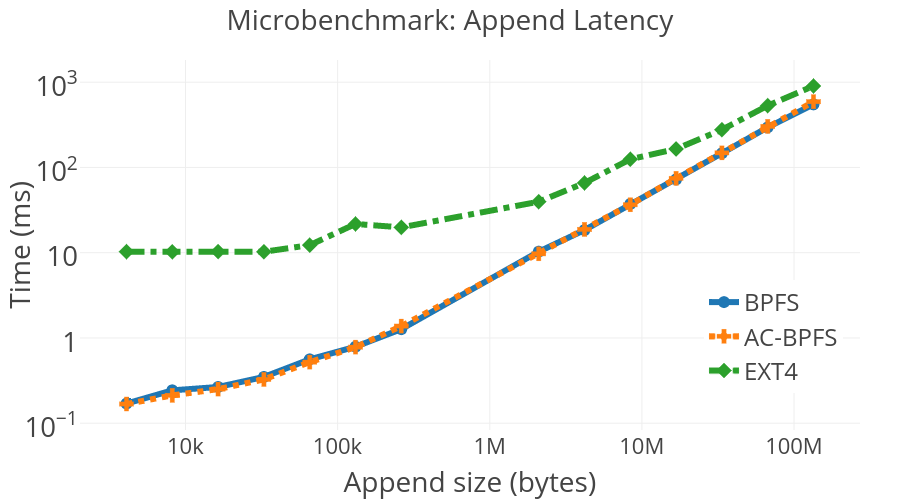
\includegraphics[width=0.5\textwidth]{figs/append.png}
\vspace{-0.1in}
\mycaption{fig-append}{Micro-benchmark: Append}{\footnotesize The figure shows the append latency for various append sizes in \textit{AC-BPFS}, \textit{BPFS} and \textit{ext4}. Note: x and y axes are in log scale.}
\end{figure}

\textbf{Analysis:} Figure~\ref{fig-append} shows that both \textit{AC-BPFS} and \textit{BPFS} perform similar and are both faster than \textit{ext4} in orders of magnitude. Append creates new data blocks and don't require cold data blocks to be fetched from disk. Since the writing of all the data for the \textit{append} operation happened entirely in NVM, \textit{AC-BPFS} and \textit{BPFS} performance lines are virtually inseparable. This result justifies the anti-caching mechanism that we have employed and also illustrates its low overhead. In our experimental setup, we set the anti-caching threshold of 40MB and hence appends of higher sizes blocks trigger eviction of blocks to disk. These evictions happen in the background and writes still go to NVM. Hence, this benchmark helps prove that the background eviction of cold blocks to disk doesn't affect the performance of \textit{AC-BPFS}.

\subsubsection{Micro-benchmark: Random Writes and Random Reads}

 \begin{figure*}[t]\centering
\begin{subfigure}{.49\textwidth}
  \centering
  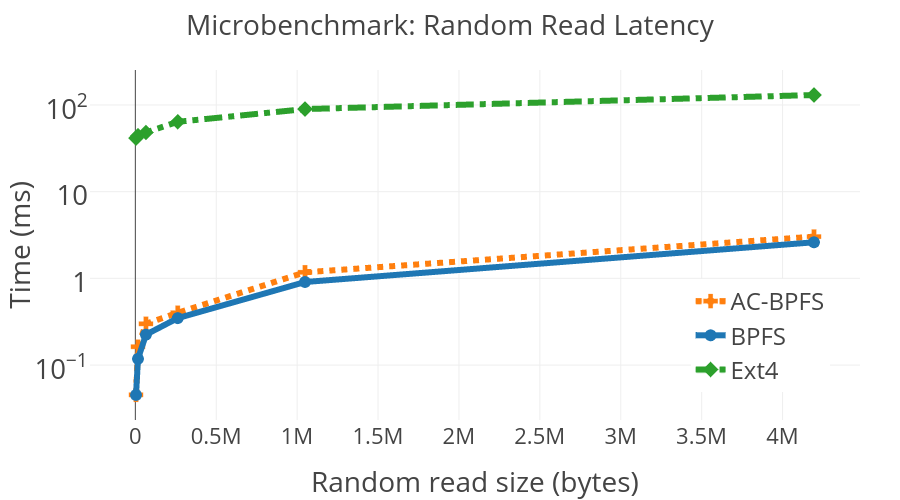
\includegraphics[width=\textwidth]{figs/read.png}
 	\centering
	\footnotesize\textit{(a) Micro-benchmark: Read}
\end{subfigure}
\begin{subfigure}{.49\textwidth}
  \centering
  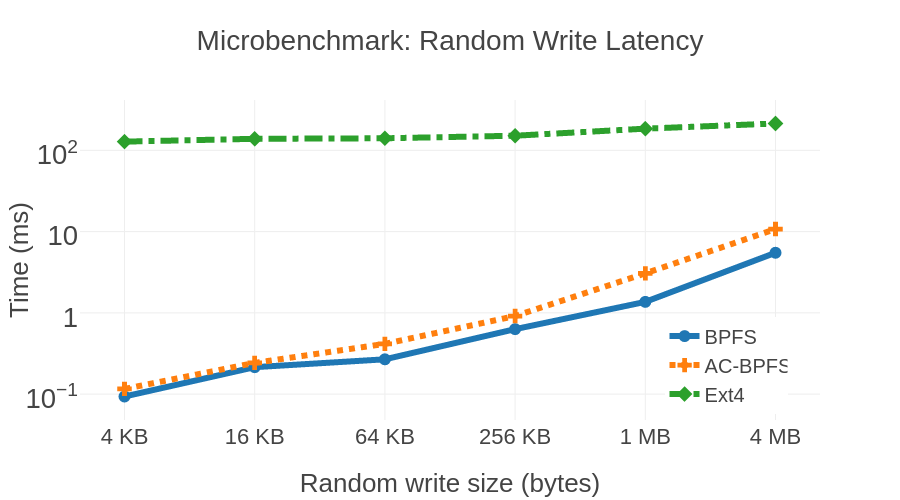
\includegraphics[width=\textwidth]{figs/write.png}
\footnotesize\textit{(b) Micro-benchmark: Write}
\end{subfigure}
\mycaption{fig-write}{Micro-benchmarks}{\footnotesize Figures (a) and (b) shows the average random read latency and average random write latency respectively for various data sizes in \textit{AC-BPFS}, \textit{BPFS} and \textit{ext4}. Note: y axis is in log scale.\\}
\end{figure*}

We evaluated the performance of making random \textit{write} and random \textit{read} operations for various data sizes for \textit{AC-BPFS}, \textit{BPFS} and \textit{ext4}. These random writes are in fact random overwrites and we dealt with appends in a separate benchmark. For \textit{AC-BPFS}, we pre-generated files of various sizes and ensured that the total size of the data set exceeded the anti-caching threshold to force eviction of blocks to disk. This ensures distribution of random read and random write operations to data blocks in both persistent memory and disk. For random writes, we called \textit{fsync} after every write call to force the data to disk so as to make even comparisons across the filesystems. Also to force random read from disk, we clear the operating system buffer cache by issuing \textit{sync}~\cite{sync} at the start of each run. This will force a seek to disk when accessing cold data in case of \textit{AC-BPFS} while forcing random reads to disk all the time in case of \textit{ext4}. We repeated each read and write operation 100 times and take the average latency for each operation.

\textbf{Analysis:} Figure~\ref{fig-write}(a) and figure~\ref{fig-write}(b) show the the plots for average time taken per random read and random write respectively for various data sizes. Since our requests are distributed across NVM and disk in case of \textit{AC-BPFS}, random reads and random overwrites of data might require fetching of data blocks from disk for few requests while most of the requests go to NVM. We do not have the exact distribution of requests to disk and NVM as we chose blocks in random. We perform a controlled experiment in the next subsection. This explains the difference in latency between \textit{AC-BPFS} and \textit{BPFS} in figures ~\ref{fig-write}(a) and ~\ref{fig-write}(b). But, both \textit{AC-BPFS} and \textit{BPFS} are still faster than the \textit{ext4} in orders of magnitude, as we hoped, thus reinforcing our initial intuition. Random writes are slower than random reads, as random overwrites of data in \textit{BPFS} and \textit{AC-BPFS} trigger shadow paging.

\subsubsection{Micro-benchmark: Degree of hotness}
This micro-benchmark demonstrates the effect of the anti-caching and plots the read latency of reading 400 KB data against the degree of hotness. As in the previous experiment, we clear the operating system buffer cache by issuing \textit{sync} at the start of each run. For the benchmark, we read a 400 KB chunk of data split into ten requests of 40KB chunk per request, part of which can be hot/cold depending on the degree of hotness. To implement this benchmark, we create 10 files of 40 KB each and we fix our anti-caching threshold based on the hotness factor, so that at any given point only the percentage of files corresponding to the hotness factor can reside in NVM. Then a workload is created, which simulates the reading of certain number of files in the NVM vs the files in the disk, based on the degree of hotness. A 20\% hotness factor on the X-axis for a 400 KB chunk data size would mean that 320 KB of the \textit{cold} data resides in disk, while 80 KB of \textit{hot} data resides in NVM for \textit{AC-BPFS}. The requests always go to disk for \textit{ext4}.

\begin{figure}
\centering
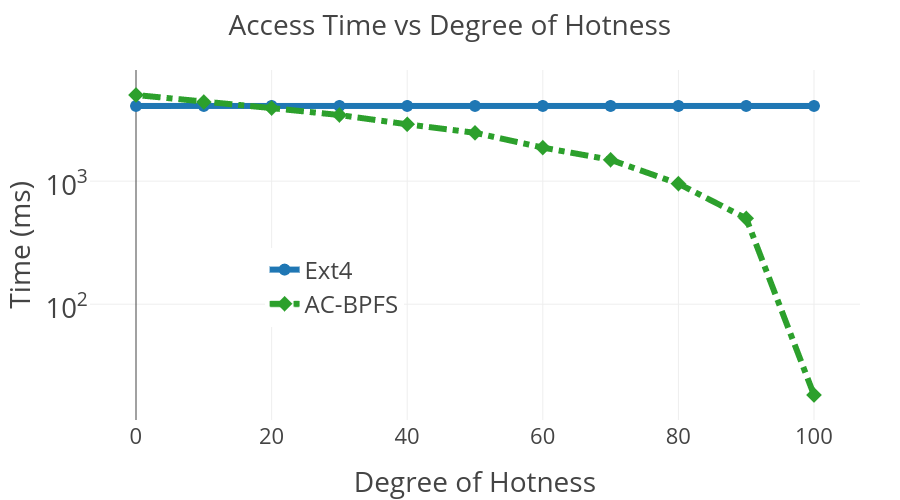
\includegraphics[width=0.5\textwidth]{figs/hotness.png}
\mycaption{fig-hotness}{Impact of Degree of Hotness on Read Latency}{\footnotesize This figure shows the read latency for various degrees of hotness in \textit{AC-BPFS} and \textit{ext4}. Note: y axis is in log scale.}
\end{figure}

\textbf{Analysis:} Figure~\ref{fig-hotness} shows the read latency for reading 400 KB data for various degrees of hotness in \textit{AC-BPFS} and \textit{ext4}. As expected, the read latency for a 20\% hot data would be more than the read latency for a 80\% hot data. At a 0\% hotness, the performance of \textit{AC-BPFS} will flat-line with the \textit{ext4} performance while at 100\% hotness our performance is exactly what you would expect from \textit{BPFS}. The more the degree of hotness, the more is the performance. This clearly proves the benefit of our anti-caching implementation for a tiered storage.

\subsection{Macro-benchmark: Filebench}
\begin{figure*}[t]\centering
\begin{subfigure}{.49\textwidth}
\centering
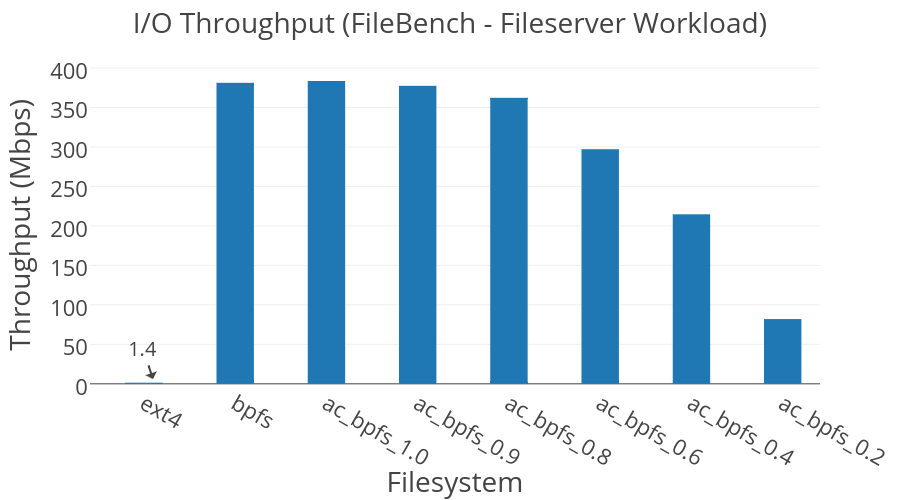
\includegraphics[width=\textwidth]{figs/filebench.png}
	\centering
\footnotesize\textit{(a) FileBench (FileServer) - I/O Throughput}
\end{subfigure}
\begin{subfigure}{.49\textwidth}
\centering
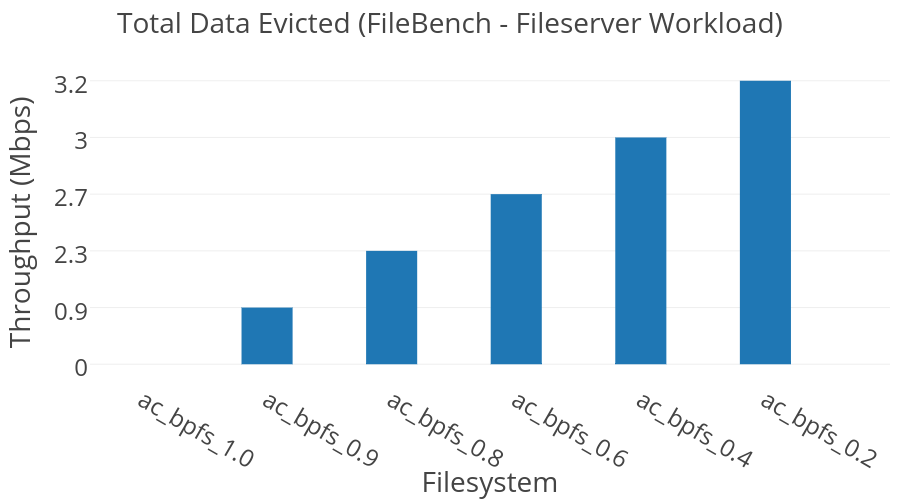
\includegraphics[width=\textwidth]{figs/bench2.png}
\footnotesize\textit{(b) FileBench (FileServer) - Block Eviction Count}
\centering
\end{subfigure}
\mycaption{fig-fb}{Macro-benchmark: FileBench (FileServer)}{\footnotesize Figure (a) shows the I/O throughput of \textit{ext4}, \textit{BPFS} and \textit{AC-BPFS} under varying anti-caching thresholds for the fileserver workload in Filebench. Figure (b) shows the total amount of data evicted from NVM to disk under various anti-caching thresholds for the FileBench fileserver workload in \textit{AC-BPFS}}
\end{figure*}

For this benchmark, we used Filebench ~\cite{filebench} to test and compare the performance in terms of overall I/O throughput of the three files systems by generating a fileserver workload on a data set of size 1.25 GB. The workload is comprised of 33\% read requests and 67\% write requests. We modified the workload to issue an \textit{fsync} after writes to make the data durable. For \textit{AC-BPFS}, we ran the benchmark by varying the anti-caching thresholds from 20\% of the workload size to 100\% of the workload size. We did so in order to get insights on the effectiveness and overheads of the anti-caching mechanisms in addition to making comparison of the \textit{AC-BPFS} with \textit{BPFS} and \textit{ext4} file systems.

\textbf{Analysis:} Figure~\ref{fig-fb}(a) shows that when the caching threshold is 100\% of the workload size (i.e. all the operations happen in the persistent memory), the performance of \textit{AC-BPFS} is identical to that of \textit{BPFS}, as we expected. As we decrease the anti-caching threshold, the performance suffers accordingly. On all times, the performance of the \textit{AC-BPFS} is better than that of \textit{ext4} on disk in orders of magnitude. Diving deeper, we measure the total data that was evicted to disk for various anti-caching thresholds. Figure~\ref{fig-fb}(b) shows the total amount of data evicted from NVM to disk under various anti-caching thresholds in \textit{AC-BPFS}. \textit{ac\_bpfs\_1.0} denotes that the anti-caching threshold was set to 100\% of workload size and hence no data was evicted to disk. At lower anti-caching threshold, more data is evicted to disk. For example at 20\% eviction threshold, close to 3GB data is evicted to disk. This is greater than the workload size of 1.25GB as fetching of cold data from disk will evicts colder data from NVM. This indicates that atleast 1.75GB of data was fetched from disk. We didn't have control over the access pattern in the workload and the requests were randomly distributed across NVM and disk and 20\% anti-caching threshold didn't correspond to 80\% access to 20\% hot data. With a 80-20 workload pattern, we believe the performance of AC-BPFS would have been better.
